%%%%%%%%%%%%%%%%%%%%%%%%%%%%%%%%%%%%%%%%%%%%%%%%%%%%%%%%%%%%%%%%%%%%%%%%%%%%%%%
%%                                                                           %%
%%   Dr Derek Harter                                                         %%
%%   Profesor, Department of Computer Science                                %% 
%%   Texas A&M University - Commerce, USA                                    %%
%%                                                                           %%
%%%%%%%%%%%%%%%%%%%%%%%%%%%%%%%%%%%%%%%%%%%%%%%%%%%%%%%%%%%%%%%%%%%%%%%%%%%%%%%
%%%%     SETTING STARTS - DO NOT CHANGE Unless your TeX setting require so   %%
%%%%%%%%%%%%%%%%%%%%%%%%%%%%%%%%%%%%%%%%%%%%%%%%%%%%%%%%%%%%%%%%%%%%%%%%%%%%%%%
%%----------------------------------------------------------------------------------
% DO NOT Change this. It is the required setting letterpaper page, 11pt, onside print, book style
%%----------------------------------------------------------------------------------
\documentclass[letterpaper,11pt,oneside]{book}

%%-------------------------------------
%% Page margin settings - % half inch margin all sides (recommended)
%%-------------------------------------
\usepackage[margin=1.2in]{geometry} 

%%-------------------------------------
%% Font settings - % CM San or Ariel (recommended)
%%-------------------------------------
% Switch the following two line off: to revert back to default LaTex font (NOT recommended)
\usepackage{amsfonts}
\renewcommand*\familydefault{\sfdefault}

%%-------------------------------------
%% Math/Definition/Theorem/Algorithm packages settings 
%%-------------------------------------
\usepackage[cmex10]{amsmath}
\usepackage{amssymb}
\usepackage{amsthm}
\newtheorem{mydef}{Definition}
\newtheorem{mytherm}{Theorem}

%%-------------------------------------
%% Algorithms/Code Listing environment settings  - 
%% Please do not change these settings
%%-------------------------------------
\usepackage{algorithm}
\usepackage{algpseudocode}
\renewcommand{\algorithmicrequire}{\textbf{Input:}}
\renewcommand{\algorithmicensure}{\textbf{Output:}}
\usepackage[utf8]{inputenc}
\usepackage{listings}
\usepackage{xcolor}
\definecolor{codegreen}{rgb}{0,0.6,0.1}
\definecolor{codegray}{rgb}{0.5,0.5,0.5}
\definecolor{codeblue}{rgb}{0.10,0.00,1.00}
\definecolor{codepurple}{rgb}{0.58,0,0.82}
\definecolor{backcolour}{rgb}{1.0,1.0,1.0}

\lstdefinestyle{mystyle}{
    backgroundcolor=\color{backcolour},   
    commentstyle=\color{codegreen},
    keywordstyle=\color{codeblue},
    numberstyle=\tiny\color{codegray},
    stringstyle=\color{codepurple},
    basicstyle=\ttfamily\footnotesize,
    breakatwhitespace=false,         
    breaklines=true,                 
    captionpos=b,                        
    keepspaces=true,                 
    numbers=left,                    
    numbersep=5pt,                  
    showspaces=false,                
    showstringspaces=false,
    showtabs=false,                  
    tabsize=2,
    frame=none
}
\lstset{style=mystyle}

%%-------------------------------------
%% Graphics/Figures environment settings
%%-------------------------------------
\usepackage{graphicx}
\usepackage{subfigure}
\usepackage{caption}
\usepackage{lipsum}

%%-------------------------------------
%% Table environment settings
%%-------------------------------------
\usepackage{multirow}
\usepackage{rotating}
\usepackage{makecell}
\usepackage{booktabs}
%\usepackage{longtable,booktabs}

%%-------------------------------------
%% List of Abbreviations settings
%%-------------------------------------
\usepackage{enumitem}
\newlist{abbrv}{itemize}{1}
\setlist[abbrv,1]{label=,labelwidth=1in,align=parleft,itemsep=0.1\baselineskip,leftmargin=!}

%%-------------------------------------
%% Bibliography/References settings   - Harvard Style was used in this report
%%-------------------------------------
\usepackage[hidelinks]{hyperref}
\usepackage[comma,authoryear]{natbib}
\renewcommand{\bibname}{References} % DO NOT remove or switch of 

%%-------------------------------------
%% Appendix settings     
%%-------------------------------------
\usepackage[toc]{appendix}
%%%%%%%%%%%%%%%%%%%%%%%%%%%%%%%%%%%%%%%%%%%%%%%%%%%%%%%%%%%%%%%%%%%%%%%%%%%%%%%%%%%%%%%
%%%%                     SETTING ENDS                                            %%%%%%
%%%%%%%%%%%%%%%%%%%%%%%%%%%%%%%%%%%%%%%%%%%%%%%%%%%%%%%%%%%%%%%%%%%%%%%%%%%%%%%%%%%%%%%
\begin{document}

    \captionsetup[figure]{margin=1.5cm,font=small,name={Figure},labelsep=colon}
    \captionsetup[table]{margin=1.5cm,font=small,name={Table},labelsep=colon}
    \SetLipsumDefault{1}
    
    \frontmatter
    
    \begin{titlepage}      
        \begin{center}
            
\includegraphics[width=3cm]{figures/tamuc-logo.png}\\[0.5cm]
            {\LARGE Texas A\&M University - Commerce\\[0.5cm]
            Department of Computer Science}\\[2cm]
			%{\color{blue} \rule{\textwidth}{1pt}}
			
			% -------------------------------
			% You need to edit some details here
			% -------------------------------  
            \linespread{1.2}\huge {
                %%%%%%%%%%%%%%%%%%%%%%%%%%%%
                %TODO: 1 TITLE of Your PROJECT 
                %%%%%%%%%%%%%%%%%%%%%%%%%%%%
                % chnage the following line                
                Comparitative Analysis of Heart Disease Detection using Standard Machine Learning Models
            
            }
            \linespread{1}~\\[2cm]
			%{\color{blue} \rule{\textwidth}{1pt}}
            {\Large 
                %%%%%%%%%%%%%%%%%%%%%%%%%%%%
                %TODO: 2 YOUR NAME
                %%%%%%%%%%%%%%%%%%%%%%%%%%%%             
                % chnage the following line
                Swetha Paspunuri
                % change end             
            }\\[1cm] 
            

            {\large 
                %%%%%%%%%%%%%%%%%%%%%%%%%%%%
                %TODO: 3 YOUR NAME Supervisor's name(s)
                %%%%%%%%%%%%%%%%%%%%%%%%%%%%             
                % change the following line                
                \emph{Supervisor:} Derek Harter, Ph.D.}\\[1cm] % if applicable
            
    		% PLEASE DO NOT CHANGE THIS TEXT %
            \large A report submitted in partial fulfilment of the requirements of\\Texas A\&M University - Commerce for the degree of\\ Master of Science in \textit{Computer Science}\\[0.3cm] 
            \vfill
            
            
            \today % Please update this date you can use \date{April 2020} for fixed date
        \end{center}
    \end{titlepage}
    
    
    % -------------------------------------------------------------------
    % Declaration
    % -------------------------------------------------------------------
    \newpage
    \thispagestyle{empty}
    \chapter*{\Large Declaration}
    % PLEASE CHANGE THIS TEXT EXCEPT YOUR NAME%
    % -------------------------------
    %TODO: PLEASE ONLY UPDATE HERE -- PLEASE WRITE YOUR NAME %    
    % ------------------------------- 
    I,
    %%%%%%%%%%%%%%%%%%%%%%%
    Swetha Paspunuri, % Mandatory part
    %%%%%%%%%%%%%%%%%%%%%%%
    of the Department of Computer Science, Texas A\&M University - Commerce, confirm that this is my own work and figures, tables, equations, code snippets, artworks, and illustrations in this report are original and have not been taken from any other person's work, except where the works of others have been explicitly acknowledged, quoted, and referenced. I understand that if failing to do so will be considered a case of plagiarism. Plagiarism is a form of academic misconduct and will be penalised accordingly. \\
    
    %% Please delete as appropriate. 
    \noindent
    %%%%%%%%%%%%%%%%%%%%%%%%%%%%%%%%%%%%%%%%%%%%%%% 
    %TODO 1 Consent for example copy -  we will use 
    I give consent to a copy of my report being shared with future students as an exemplar. \\
    
    \noindent
    %%%%%%%%%%%%%%%%%%%%%%%%%%%%%%%%%%%%%%%%%%%%%%% 
    %TODO 2 Consent to let the report to use use by library for public use
    I give consent for my work to be made available more widely to members of TAMUC and public with interest in teaching, learning and research. 
    %%%%%%%%%%%%%%%%%%%%%%%%%%%%%%%%%%%%%%%%%%%%%%%
    ~\\[1cm]
    \begin{flushright}
	%------------------------------ 
	% change the following line
    %TODO: PLEASE UPDATE  Your Name  -------------------------------%
	Swetha Paspunuri % Please change it to your name
    
    \today
    \end{flushright}

     
    % -------------------------------------------------------------------
    % Abstract and Acknowledgement
    % -------------------------------------------------------------------
    
    %Two resources useful for abstract writing.
% Guidance of how to write an abstract/summary provided by Nature: https://cbs.umn.edu/sites/cbs.umn.edu/files/public/downloads/Annotated_Nature_abstract.pdf %https://writingcenter.gmu.edu/guides/writing-an-abstract
\chapter*{\center \Large  Abstract}
%%%%%%%%%%%%%%%%%%%%%%%%%%%%%%%%%%%%%%
% Replace all text with your text
%%%%%%%%%%%%%%%%%%%%%%%%%%%%%%%%%%%
In Contemporary world Cardiovascular diseases have seen a rise, even affecting newborn. Detecting heart-related diseases prior is vital because it helps doctors start treatment sooner, leading to better results for patients and less strain on healthcare resources. With more and more people facing heart problems, it's crucial to have advanced predictive tools. Using the abundant data available in Cardiology, our project aims to integrate the technology into health care for predictive modelling. The primary goal of this project is to develop an efficient heart disease prediction system using various machine learning models to predict Coronary Artery Disease with utmost precision and effectiveness. We employed a dataset consisting of necessary patient information from online sources to train and validate our models. The first step is Cleaning and preprocessing data that allow us to find key patterns for training the models. The various machine learning models used are Logistic Regression, Random Forest, Naive Bayes. We evaluate these models using important measures like precision, which tells us how accurate positive predictions are; recall, which shows how well the models capture all actual positive cases; and the F1 score, which balances both precision and recall which can be assessed to provide the health sectors with a more efficient approach to detect heart related diseases.



%%%%%%%%%%%%%%%%%%%%%%%%%%%%%%%%%%%%%%%%%%%%%%%%%%%%%%%%%%%%%%%%%%%%%%%%%s
~\\[1cm]
\noindent % Provide your key words
\textbf{Keywords:} Logistic Regression, Random Forest, Naive Bayes , F1 score,Precision.


\vfill
\noindent
\textbf{Report's total word count:} we expect a maximum of 10,000 words (excluding reference and appendices) and about 10 pages. [A good project report can also be written in approximately 5,000 words.]


    % -------------------------------------------------------------------
	% Acknowledgement
	% -------------------------------------------------------------------
   
    \chapter*{\center \Large  Acknowledgements}
%%%% Update with your text %%%%%%%%%%%%%%%
An acknowledgements section is optional. You may like to acknowledge the support and help of your supervisor(s), friends, or any other person(s), department(s), institute(s), etc. If you have been provided specific facility from department/school acknowledged so.  

   
    
    % -------------------------------------------------------------------
    % Contents, list of figures, list of tables
    % -------------------------------------------------------------------
    
    \tableofcontents
    \listoffigures
    \listoftables
    \chapter*{List of Abbreviations}
\chaptermark{List of Abbreviations}
%%%%%%%%%%%%%%%%%%%%%%%%%%%%%%%%%%%
%%  Enter your list of Abbreviation and Symbols in this file
%%%%%%%%%%%%%%%%%%%%%%%%%%%%%%%%%%%
\begin{abbrv}
    \item[LR]			Logistic Regression
    \item[RF]			Random Forest
    \item[NB]			Naive Bayes
    \item[CAD]           Coronary Artery 
Disease
\end{abbrv}
 %  Enter your list of Abbreviation and Symbols in this file
    
    %%%%%%%%%%%%%%%%%%%%%%%%%%%%%%%%%%%%%%%%%%%%%%%%%%%%%%%%%%%%%%%%%%%%%%%%
    %%                                                                    %%  
    %%  Main chapters and sections of your project                        %%  
    %%  Everything from here on needs updates in your own words and works %%
    %%                                                                    %%
    %%%%%%%%%%%%%%%%%%%%%%%%%%%%%%%%%%%%%%%%%%%%%%%%%%%%%%%%%%%%%%%%%%%%%%%%
    \mainmatter
    % Read for preparation of document in LaTex 
    % Lamport, L. (1986), LATEX: A Document Preparation System, Addison-Wesley.
    
    \chapter{Introduction}
\label{ch:into} % This how you label a chapter and the key (e.g., ch:into) will be used to refer this chapter ``Introduction'' later in the report. 
% the key ``ch:into'' can be used with command \ref{ch:intor} to refere this Chapter.
Today, heart problems are a major health concern affecting individuals worldwide. Many people are suffering from heart issues like heart disease, heart failure, and irregular heartbeats nowadays. Heart problems can affect people, not just physically but also emotionally. Those with heart conditions often find it difficult to live normally and face many difficulties. Additionally, the financial side of managing heart problems adds an extra layer of challenges. Spotting heart-related issues early is crucial. It helps healthcare professionals to step in quickly, enhance patient outcomes, and ease the strain on healthcare resources. Early detection allows for timely intervention, potentially preventing the progression of heart conditions.To address the need for early detection, our project focuses on developing a machine learning model capable of accurately identifying the presence of heart diseases. In this endeavor, we utilize a heart-related issue dataset from \citep{janosi-1988}, sourced from the online repository UC Irvine. The data undergoes thorough cleaning and pre-processing to extract useful information essential for training the machine learning model. The machine learning algorithms employed, as highlighted by \citep{Sharma-2020}, include Logistic Regression, Naïve Bayes, and Random Forest classification. These algorithms have demonstrated effectiveness in detecting coronary artery disease by evaluating outputs based on various factors such as resting blood pressure, serum cholesterol, maximum heart rate achieved, and more. Furthermore, our project aims not only to detect heart-related issues but also to contribute valuable insights to the broader field of cardiovascular health. By leveraging advanced algorithms, we seek to ensure the effective prediction of heart-related problems, potentially revolutionizing the early diagnosis and management of cardiovascular conditions.
%%%%%%%%%%%%%%%%%%%%%%%%%%%%%%%%%%%%%%%%%%%%%%%%%%%%%%%%%%%%%%%%%%%%%%%%%%%%%%%%%%%
\section{Background}
\label{sec:into_back}
Our project focuses on addressing the issue of cardiovascular diseases in today's world, affecting everyone irrespective of their age. The primary motivation behind our work is to detect the heart-related diseases as early as possible. This identification helps doctors to start the treatment sooner, to improve patient results and effectively using the healthcare resources. For this, our project focuses on integrating technology into healthcare by using the abundant data in cardiology for predictive modeling. The primary goal is to develop an efficient heart disease prediction system by concentrating on predicting Coronary Artery Disease with precision and effectiveness. So, we use different machine learning models such as Logistic Regression, Random Forest, and Naive Bayes. These models play a crucial role in predicting and understanding heart-related issues. The initial phase involves cleaning and preprocessing the data to extract necessary patterns required for training the models. Our project becomes significant as it can give better resources to doctors for finding and handling heart problems early on. We want to help make hearts healthier by explaining some crucial ideas and ways to use them in a simple way.

%%%%%%%%%%%%%%%%%%%%%%%%%%%%%%%%%%%%%%%%%%%%%%%%%%%%%%%%%%%%%%%%%%%%%%%%%%%%%%%%%%%
\section{Research Question}
\label{sec:intro_prob_art}
Prediction of Heart Disease(Cardiovascular) Using Machine Learning Algorithms such as Logistic Regression, Random Forest, and Naive Bayes.

%%%%%%%%%%%%%%%%%%%%%%%%%%%%%%%%%%%%%%%%%%%%%%%%%%%%%%%%%%%%%%%%%%%%%%%%%%%%%%%%%%%
\section{Aims and objectives}
\label{sec:intro_aims_obj}
 

\textbf{Aims:}To develop and implement an advanced heart disease prediction system, utilizing machine learning models for early detection of Coronary Artery Disease, with the ultimate goal of enhancing patient outcomes and contributing to the ongoing global efforts in cardiovascular health.
\textbf{Objectives:} The Objectives include to Perform data cleaning and preprocessing, apply Logistic Regression, Naïve Bayes, and Random Forest algorithms, integrate technology into healthcare, provide valuable resources to healthcare professionals, and innovate existing approaches to address gaps, thereby achieving early identification and proactive management of heart-related issues.



%%%%%%%%%%%%%%%%%%%%%%%%%%%%%%%%%%%%%%%%%%%%%%%%%%%%%%%%%%%%%%%%%%%%%%%%%%%%%%%%%%%
\section{Solution approach}
\label{sec:intro_sol} % label of Org section
Briefly describe the solution approach and the methodology applied in solving the set aims and objectives.

Depending on the project, you may like to alter the ``heading'' of this section. Check with you supervisor. Also, check what subsection or any other section that can be added in or removed from this template.

\subsection{A subsection 1}
\label{sec:intro_some_sub1}
You may or may not need subsections here. Depending on your project's needs, add two or more subsection(s). A section takes at least two subsections. 

\subsection{A subsection 2}
\label{sec:intro_some_sub2}
Depending on your project's needs, add more section(s) and subsection(s).

\subsubsection{A subsection 1 of a subsection}
\label{sec:intro_some_subsub1}
The command \textbackslash subsubsection\{\} creates a paragraph heading in \LaTeX.

\subsubsection{A subsection 2 of a subsection}
\label{sec:intro_some_subsub2}
Write your text here...

%%%%%%%%%%%%%%%%%%%%%%%%%%%%%%%%%%%%%%%%%%%%%%%%%%%%%%%%%%%%%%%%%%%%%%%%%%%%%%%%%%%
\section{Summary of contributions and achievements} %  use this section 
\label{sec:intro_sum_results} % label of summary of results
Describe clearly what you have done/created/achieved and what the major results and their implications are. 


%%%%%%%%%%%%%%%%%%%%%%%%%%%%%%%%%%%%%%%%%%%%%%%%%%%%%%%%%%%%%%%%%%%%%%%%%%%%%%%%%%%
\section{Organization of the report} %  use this section
\label{sec:intro_org} % label of Org section
Describe the outline of the rest of the report here. Let the reader know what to expect ahead in the report. Describe how you have organized your report. 

\textbf{Example: how to refer a chapter, section, subsection}. This report is organised into seven chapters. Chapter~\ref{ch:lit_rev} details the literature review of this project. In Section~\ref{ch:method}...  % and so on.

\textbf{Note:}  Take care of the word like ``Chapter,'' ``Section,'' ``Figure'' etc. before the \LaTeX command \textbackslash ref\{\}. Otherwise, a  sentence will be confusing. For example, In \ref{ch:lit_rev} literature review is described. In this sentence, the word ``Chapter'' is missing. Therefore, a reader would not know whether 2 is for a Chapter or a Section or a Figure.


    \chapter{Literature Review}
\label{ch:lit_rev} %Label of the chapter lit rev. The key ``ch:lit_rev'' can be used with command \ref{ch:lit_rev} to refer this Chapter.
The literature review looks into the current state of cardiovascular disease research, highlighting its global impact across different age groups. Many recent studies show worry about heart problems like disease, failure, and abnormal rhythms, which hurt people's bodies and emotions. Identifying the health issues sooner could help the doctors to respond fast, improve the patient results, effectively utilize the health care resources. [4] Janosi and Detrano's (1988) heart-related issue dataset from UC Irvine serves as a valuable resource for our project, showing how existing data can be helpful in medicine. [5] The study by Sharma et al. (2020) reinforces the significance of employing machine learning algorithms, specifically Logistic Regression, Naïve Bayes, and Random Forest classification, for accurate detection of coronary artery disease. Studies show that things like how high your blood pressure is at rest, how much cholesterol you have in your blood (serum cholesterol), and how fast your heart beats during exercise are all important for figuring out if someone might have heart disease. Our project mainly focuses on integrating technology into healthcare, aligning with the existing literature. [6] Looking at past research on heart disease prediction shows what are the necessary improvements and different ways to predict and understand heart problems. By addressing these gaps, our project helps doctors find and treat heart problems as soon as possible, which is btter for patients and hospitals. The literature review emphasizes our significant impact in contributing to the ongoing efforts to combat cardiovascular diseases and underscores the need for advanced predictive tools to address this global health challenge.

% PLEAE CHANGE THE TITLE of this section
\section{Example of ``risk'' of unintentional plagiarism}
Using other sources, ideas, and material always bring with it a risk of unintentional plagiarism. 

\noindent
\textbf{\color{red}MUST}: do read the university guidelines on the definition of plagiarism as well as the guidelines on how to avoid plagiarism~\citep{uor_plagiarism}.




% A possible section of you chapter
\section{Critique of the review} % Use this section title or choose a betterone
Describe your main findings and evaluation of the literature. ~\\

% Pleae use this section
\section{Summary} 
Write a summary of this chapter~\\
% https://guides.library.bloomu.edu/litreview
    % replace all text with your own text.
% in this template few examples are mention
\chapter{Methodology}
\label{ch:method} % Label for method chapter
Recognizing the need for early detection and management of cardiovascular conditions, we utilize machine learning algorithms to analyze patient data and predict the likelihood of heart disease. Our methodology encompasses data collection, preprocessing, feature extraction, model development, and evaluation, aiming to deliver a robust and effective predictive tool for doctors. By integrating innovative learning algorithms and conducting experiments, we aspire to contribute meaningful solutions and enhance patient outcomes in cardiovascular health.

\section{Algorithms Descriptions}
\subsection{Logistic Regression}
LR is a statistical method used for binary classification tasks. It models the probability of a binary outcome based on one or more predictor variables. In the context of heart disease prediction, LR can analyze patient parameters such as age, cholesterol levels, and blood pressure to estimate the likelihood of the presence of heart disease.

\subsection{Naïve Bayes}
NB is a probabilistic classifier based on Bayes' theorem with an assumption of independence between features. In heart disease prediction, Naïve Bayes can effectively analyze patient attributes and calculate the conditional probability of heart disease given the observed features. Its simplicity and computational efficiency make Naïve Bayes a popular choice for healthcare applications.

\subsection{Random Forest}
RF is an ensemble learning method that constructs a multitude of decision trees during training and outputs the mode of the classes (classification) or mean prediction (regression) of the individual trees. In heart disease prediction, Random Forest can analyze a large number of patient parameters and identify complex patterns associated with cardiovascular conditions.

\section{Implementations}
\subsection{Logistic Regression}
For LR implementation, we'll utilize the `LogisticRegression` class from the `sklearn.linear\_model` module. We'll preprocess the dataset, including handling missing values and scaling features, before fitting the model to the training data.
\subsection{Naïve Bayes}
For NB implementation, we'll use the `GaussianNB` class from the `sklearn.naive\_bayes` module. Similar to Logistic Regression, we'll preprocess the dataset and fit the model to the training data.
\subsection{Random Forest}
For RF implementation, we'll employ the `RandomForestClassifier` class from the `sklearn.ensemble` module. We'll preprocess the dataset and tune hyperparameters, such as the number of estimators and maximum depth, to optimize model performance.

\section{Experiments Design}
In our experimental approach to assess the predictive performance of each algorithm for heart disease, we'll begin by dividing our dataset into separate training and testing sets. This division ensures that the models are trained on a subset of the data and evaluated on an independent portion, enabling us to gauge their generalization capability. To further fortify the reliability of our findings, we'll employ cross-validation techniques. This involves iteratively partitioning the dataset into multiple subsets, training the models on different combinations, and validating them on the remaining data, thus providing a more comprehensive evaluation. Subsequently, we'll utilize a range of performance metrics, including accuracy, precision, recall, and F1-score, to quantify the algorithms' effectiveness. These metrics will allow us to discern not only the models' overall correctness but also their ability to precisely identify positive cases and recall them accurately. By meticulously analyzing these performance indicators, we aim to determine the most optimal approach for heart disease prediction, considering factors such as model interpretability and computational efficiency alongside predictive accuracy.

\section{Algorithms}
In our project, we implement three distinct machine learning algorithms—Logistic Regression, Random Forest, and Naive Bayes—to predict heart disease. Logistic Regression is a simple yet powerful algorithm used for binary classification tasks, where it models the probability of a binary outcome. Random Forest, on the other hand, is an ensemble learning method that constructs multiple decision trees and aggregates their predictions to improve accuracy. Naive Bayes is a probabilistic classifier based on Bayes' theorem, particularly effective for datasets with high dimensionality and strong feature independence assumptions. Each algorithm offers unique advantages and approaches in identifying patterns and making predictions, contributing to our comprehensive analysis of heart disease prediction.

\begin{algorithm}
    \caption{Logistic Regression}
    \label{algo:logistic_regression}
    \begin{algorithmic}[1]
        \Require{Training dataset $(X_{train}, Y_{train})$, Test dataset $X_{test}$}
        \Ensure{Predicted class labels for $X_{test}$}
        \Statex
        \Function{LogisticRegression}{$X_{train}, Y_{train}, X_{test}$}
        \State Initialize logistic regression classifier
        \State Standardize features: $X_{train} \gets \text{StandardScaler.fit\_transform}(X_{train})$
        \State Fit classifier to training data: $classifier.fit(X_{train}, Y_{train})$
        \State Standardize test features: $X_{test} \gets \text{StandardScaler.transform}(X_{test})$
        \State Predict probabilities for test data: $y_{prob} \gets classifier.predict\_proba(X_{test})$
        \State Convert probabilities to class labels: $y_{pred} \gets \text{threshold\_function}(y_{prob})$
        \State \Return $y_{pred}$
        \EndFunction
    \end{algorithmic}
\end{algorithm}

\begin{algorithm}
    \caption{Random Forest}
    \label{algo:random_forest}
    \begin{algorithmic}[1]
        \Require{Training dataset $(X_{train}, Y_{train})$, Test dataset $X_{test}$}
        \Ensure{Predicted class labels for $X_{test}$}
        \Statex
        \Function{RandomForest}{$X_{train}, Y_{train}, X_{test}$}
        \State Initialize random forest classifier with specified parameters
        \State Handle missing values: $X_{train}, X_{test} \gets \text{Imputer.fit\_transform}(X_{train}, X_{test})$
        \State Fit classifier to training data: $classifier.fit(X_{train}, Y_{train})$
        \State Predict class labels for test data: $y_{pred} \gets classifier.predict(X_{test})$
        \State \Return $y_{pred}$
        \EndFunction
    \end{algorithmic}
\end{algorithm}

\begin{algorithm}
    \caption{Naive Bayes}
    \label{algo:naive_bayes}
    \begin{algorithmic}[1]
        \Require{Training dataset $(X_{train}, Y_{train})$, Test dataset $X_{test}$}
        \Ensure{Predicted class labels for $X_{test}$}
        \Statex
        \Function{NaiveBayes}{$X_{train}, Y_{train}, X_{test}$}
        \State Initialize naive Bayes classifier
        \State Discretize continuous features: $X_{train}, X_{test} \gets \text{Binarizer.fit\_transform}(X_{train}, X_{test})$
        \State Fit classifier to training data: $classifier.fit(X_{train}, Y_{train})$
        \State Predict class labels for test data: $y_{pred} \gets classifier.predict(X_{test})$
        \State \Return $y_{pred}$
        \EndFunction
    \end{algorithmic}
\end{algorithm}


\begin{figure}
    \centering
    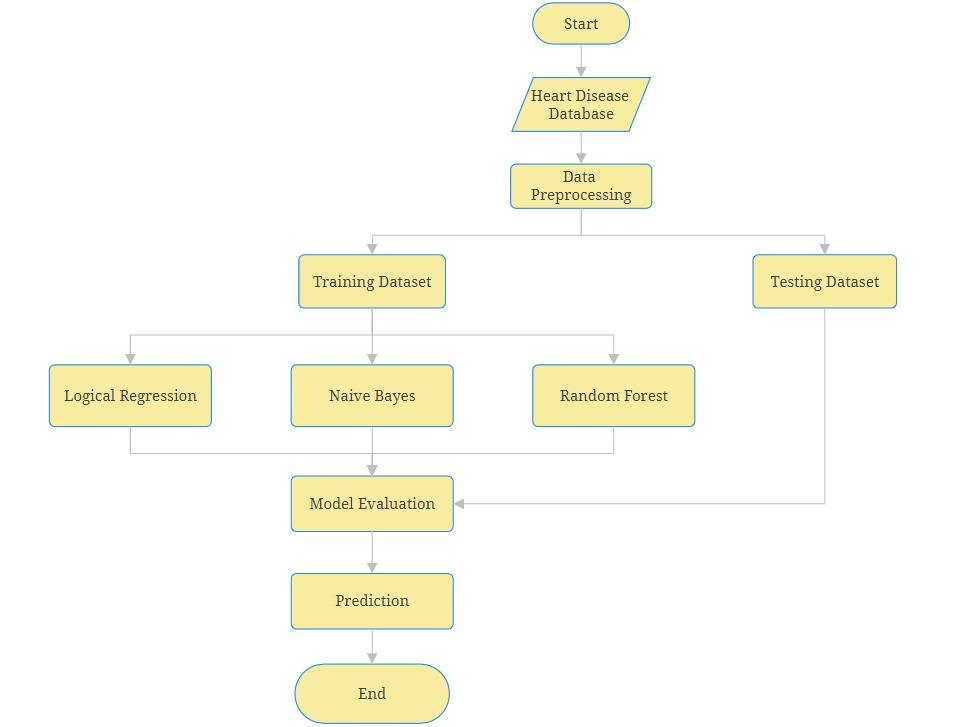
\includegraphics[width=1\linewidth]{figures/Flowchart.jpg}
    \caption{Flowchart of Heart Disease Prediction using LR, RF and NB}
    \label{fig:enter-label}
\end{figure}


\section{Code}
\subsection{Data Pre-processing}
\begin{lstlisting}[language=Python, label=list:python_code_ex]
# Importing the libraries

import numpy as np
import matplotlib.pyplot as plt
import pandas as pd

from sklearn.impute import SimpleImputer
from sklearn.model_selection import train_test_split
from sklearn.preprocessing import StandardScaler
from sklearn.metrics import accuracy_score
from sklearn.metrics import confusion_matrix
from sklearn.metrics import classification_report
from sklearn.metrics import roc_auc_score
from sklearn.metrics import roc_curve

# Importing the dataset
dataset = pd.read_csv('cleve.csv')

#defining X values ang y values
X = dataset.iloc[:, :-1].values
Y = dataset.iloc[:, 13].values

#handling missing data
imputer= SimpleImputer(missing_values=np.nan, strategy='mean')
imputer=imputer.fit(X[:,11:13])
X[:,11:13]=imputer.transform(X[:,11:13])

#splitting dataset into training set and test set
X_train,X_test,Y_train,Y_test=train_test_split(X, Y, test_size = 0.25, random_state = 101)

#feature scaling
s=StandardScaler()
X_train=s.fit_transform(X_train)
X_test=s.transform(X_test)
\end{lstlisting}

\clearpage  %

\subsection{Logistic Regression}
\begin{lstlisting}[language=Python, label=list:python_code_ex]
#fitting LR to training set
from sklearn.linear_model import LogisticRegression
LogisticRegressionClassifier =LogisticRegression()
LogisticRegressionClassifier.fit(X_train,Y_train)

#Predict the test set results
Y_pred=LogisticRegressionClassifier.predict(X_test)

#checking the accuracy for predicted results
accuracy_score(Y_test,Y_pred)

# Making the Confusion Matrix
cm = confusion_matrix(Y_test, Y_pred)

#Interpretation:
print(classification_report(Y_test, Y_pred))
\end{lstlisting}

\begin{table}[h!]
    \centering
    \caption{Classification Report of LR}
    \label{tab:_ex_tab}
    \begin{tabular}{ccccc}     
        \toprule
            &  precision & recall & f1-score & support \\
        \midrule
        0 & 0.81 & 0.94 & 0.87 & 36 \\
        1 & 0.94 & 0.80 & 0.86 & 40 \\

        accuracy & - & - & 0.87 & 76 \\
        macro avg & 0.88 & 0.87 & 0.87 & 76 \\
        weighted avg & 0.88 & 0.87 & 0.87 & 76 \\
        \bottomrule
    \end{tabular}
\end{table}

\begin{lstlisting}[language=Python, label=list:python_code_ex]
#ROC
logit_roc_auc = roc_auc_score(Y_test, LogisticRegressionClassifier.predict(X_test))
fpr, tpr, thresholds = roc_curve(Y_test, LogisticRegressionClassifier.predict_proba(X_test)[:,1])
plt.figure()
plt.plot(fpr, tpr, label='Logistic Regression (area = %0.2f)' % logit_roc_auc)
plt.plot([0, 1], [0, 1],'r--')
plt.xlim([0.0, 1.0])
plt.ylim([0.0, 1.05])
plt.xlabel('False Positive Rate')
plt.ylabel('True Positive Rate')
plt.title('Receiver operating characteristic')
plt.legend(loc="lower right")
plt.savefig('Log_ROC')
plt.show()

#PREDICTION FOR NEW DATASET using LogisticRegressionClassifier
Newdataset = pd.read_csv('newdata.csv')
ynew=LogisticRegressionClassifier.predict(Newdataset)
print("Predicted Class for newdata.csv:",ynew)
\end{lstlisting}

\begin{figure}
    \centering
    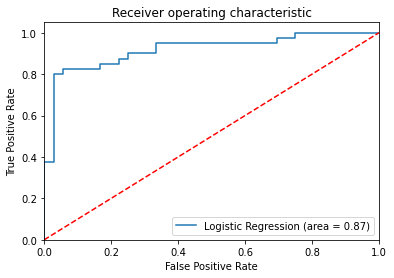
\includegraphics[width=0.5\linewidth]{LR.png}
    \caption{Receiver operating characteristics of LR}
    \label{fig:enter-label}
\end{figure}

\subsection{Random Forest}
\begin{lstlisting}[language=Python, label=list:python_code_ex]
# Fitting RandomForestClassifier to the Training set
from sklearn.ensemble import RandomForestClassifier
RandomForestClassifier =RandomForestClassifier(n_estimators=20)
RandomForestClassifier.fit(X_train, Y_train)

# Predicting the Test set results
Y_pred2 = RandomForestClassifier.predict(X_test)
from sklearn.metrics import accuracy_score
accuracy_score(Y_test,Y_pred2)

# Making the Confusion Matrix
from sklearn.metrics import confusion_matrix
cm = confusion_matrix(Y_test, Y_pred2)

#Interpretation:
print(classification_report(Y_test, Y_pred2))
\end{lstlisting}

\begin{table}[h!]
    \centering
    \caption{Classification Report of RF}
    \label{tab:_ex_tab}
    \begin{tabular}{ccccc}     
        \toprule
            &  precision & recall & f1-score & support \\
        \midrule
        0 & 0.80 & 0.89 & 0.84 & 36 \\
        1 & 0.89 & 0.80 & 0.84 & 40 \\

        accuracy & - & - & 0.84 & 76 \\
        macro avg & 0.84 & 0.84 & 0.84 & 76 \\
        weighted avg & 0.85 & 0.84 & 0.84 & 76 \\
        \bottomrule
    \end{tabular}
\end{table}

\clearpage  %

\begin{lstlisting}[language=Python, label=list:python_code_ex]
#ROC
from sklearn.metrics import roc_auc_score
from sklearn.metrics import roc_curve
logit_roc_auc = roc_auc_score(Y_test, RandomForestClassifier.predict(X_test))
fpr, tpr, thresholds = roc_curve(Y_test, RandomForestClassifier.predict_proba(X_test)[:,1])
plt.figure()
plt.plot(fpr, tpr, label='Random Forest (area = %0.2f)' % logit_roc_auc)
plt.plot([0, 1], [0, 1],'r--')
plt.xlim([0.0, 1.0])
plt.ylim([0.0, 1.05])
plt.xlabel('False Positive Rate')
plt.ylabel('True Positive Rate')
plt.title('Receiver operating characteristic')
plt.legend(loc="lower right")
plt.savefig('RF_ROC')
plt.show()

#PREDICTION FOR NEW DATASET using RandomForest
ynew=RandomForestClassifier.predict(Newdataset)
print("Predicted Class for newdata.csv:",ynew)
\end{lstlisting}

\begin{figure}[H]
    \centering
    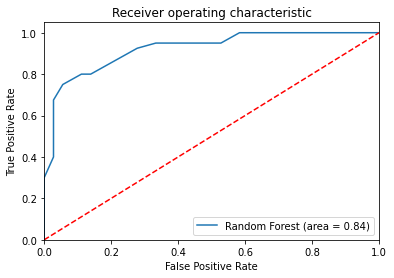
\includegraphics[width=0.5\linewidth]{RF.png}
    \caption{Receiver operating characteristics of RF}
    \label{fig:enter-label}
\end{figure}

\subsection{Naive Bayes}
\begin{lstlisting}[language=Python, label=list:python_code_ex]
NaiveBayesimputer= SimpleImputer(strategy='mean')
NaiveBayesimputer=NaiveBayesimputer.fit(X[:,11:13])
X[:,11:13]=NaiveBayesimputer.transform(X[:,11:13])

#splitting dataset into training set and test set
X_train,X_test,Y_train,Y_test=train_test_split(X, Y, test_size = 0.25, random_state = None)

# Fitting Naive Bayes to the Training set
from sklearn.naive_bayes import GaussianNB
NaiveBayesClassifier = GaussianNB()
NaiveBayesClassifier.fit(X_train, Y_train)


# Predicting the Test set results
Y_pred3 = NaiveBayesClassifier.predict(X_test)
#ACCURACY SCORE
accuracy_score(Y_test,Y_pred3)

# Making the Confusion Matrix
cm = confusion_matrix(Y_test, Y_pred3)

#Interpretation:
print(classification_report(Y_test, Y_pred3))
\end{lstlisting}

\begin{table}[h!]
    \centering
    \caption{Classification Report of NB}
    \label{tab:_ex_tab}
    \begin{tabular}{ccccc}     
        \toprule
            &  precision & recall & f1-score & support \\
        \midrule
        0 & 0.80 & 0.90 & 0.84 & 39 \\
        1 & 0.88 & 0.76 & 0.81 & 37 \\

        accuracy & - & - & 0.83 & 76 \\
        macro avg & 0.84 & 0.83 & 0.83 & 76 \\
        weighted avg & 0.83 & 0.83 & 0.83 & 76 \\
        \bottomrule
    \end{tabular}
\end{table}


\begin{lstlisting}[language=Python, label=list:python_code_ex]
#ROC
logit_roc_auc = roc_auc_score(Y_test,NaiveBayesClassifier.predict(X_test))
fpr, tpr, thresholds = roc_curve(Y_test, NaiveBayesClassifier.predict_proba(X_test)[:,1])
plt.figure()
plt.plot(fpr, tpr, label='Navie Bayes (area = %0.2f)' % logit_roc_auc)
plt.plot([0, 1], [0, 1],'r--')
plt.xlim([0.0, 1.0])
plt.ylim([0.0, 1.05])
plt.title('Receiver operating characteristic')
plt.legend(loc="lower right")
plt.savefig('NB_ROC')
plt.show()

#PREDICTION FOR NEW DATASET using NaiveBayesClassifier
ynew = NaiveBayesClassifier.predict(Newdataset)
print("Predicted Class for newdata.csv:", ynew)
\end{lstlisting}

\begin{figure}[H]
    \centering
    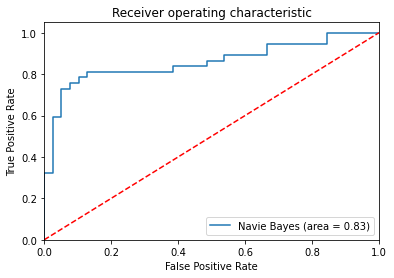
\includegraphics[width=0.4\linewidth]{NB.png}
    \caption{Receiver operating characteristics of NB}
    \label{NB}
\end{figure}
    \chapter{Results}
In this project, we aimed to develop machine learning models to predict the likelihood of heart disease in patients. We utilized three well-established algorithms: Logistic Regression, Random Forest, and Naive Bayes. The models were trained and evaluated on a dataset containing patient information relevant to heart disease.

\section{Performance Metrics:}
The performance of the models was assessed using the following metrics:

\begin{itemize}
    \item Accuracy: Overall correctness of the predictions (correctly classified instances / total instances).
    
    \item Precision: Proportion of true positives among predicted positives (true positives / (true positives + false positives)).
    
    \item: Proportion of true positives identified by the model (true positives / (true positives + false negatives)).

    \item: F1-Score: Harmonic mean of precision and recall (2 * (precision * recall) / (precision + recall)).

    \item: ROC AUC Score: Area Under the Receiver Operating Characteristic Curve (ROC) that measures the model's ability to distinguish between positive and negative cases.
    
\end{itemize}


\clearpage
\section{Results for Each Model:}
\subsection{LR Results:}
We implemented a Logistic Regression model to predict heart disease. The model achieved an accuracy of 87\%, precision of 88\% for positive cases (identifying patients with heart disease), recall of 87\% for positive cases (correctly identifying patients with heart disease), and F1-score of 87\%.


\begin{table}[h!]
    \centering
    \caption{LR Performance}
    \label{tab:_ex_tab}
    \begin{tabular}{cccc}     
        \toprule
             Metric  & Value\\
        \midrule
            Accuracy  & 87\% \\
           Precision & 88\% \\
           Recall  & 87\% \\
           F1-Score & 88\% \\ 
        \bottomrule
    \end{tabular}
\end{table}

\subsection{ROC Curve for LR}

\begin{figure}[H]
    \centering
    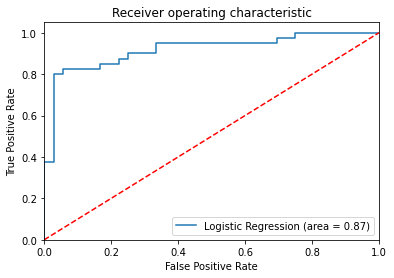
\includegraphics[width=0.5\linewidth]{LR.png}
    \caption{ROC Curve for LR}
    \label{LR}
\end{figure}

\subsection{RF Results:}
A Random Forest model was also employed for heart disease prediction. The Random Forest model achieved an accuracy of 84\%, precision of 85\% for positive cases, recall of 84\% for positive cases, and F1-score of 84\%.


\begin{table}[h!]
    \centering
    \caption{RF Performance}
    \label{tab:_ex_tab}
    \begin{tabular}{cccc}     
        \toprule
             Metric  & Value\\
        \midrule
            Accuracy  & 84\% \\
           Precision & 85\% \\
           Recall  & 84\% \\
           F1-Score & 84\% \\ 
        \bottomrule
    \end{tabular}
\end{table}

\subsection{ROC Curve for RF}

\begin{figure}[H]
    \centering
    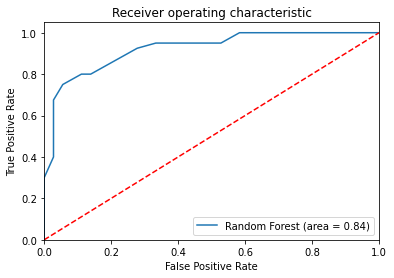
\includegraphics[width=0.5\linewidth]{RF.png}
    \caption{ROC Curve for RF}
    \label{RF}
\end{figure}

\subsection{NB Results:}
The Naive Bayes model was implemented as another approach for heart disease prediction. The Naive Bayes model achieved an accuracy of 83\%, precision of 83\% for positive cases, recall of 83\% for positive cases, and F1-score of 83\%.


\begin{table}[h!]
    \centering
    \caption{NB Performance}
    \label{tab:_ex_tab}
    \begin{tabular}{cccc}     
        \toprule
             Metric  & Value\\
        \midrule
            Accuracy  & 83\% \\
           Precision & 83\% \\
           Recall  & 83\% \\
           F1-Score & 83\% \\ 
        \bottomrule
    \end{tabular}
\end{table}

\subsection{ROC Curve for NB}

\begin{figure}[H]
    \centering
    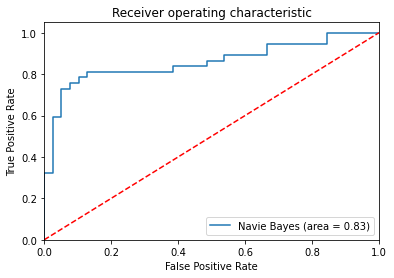
\includegraphics[width=0.5\linewidth]{NB.png}
    \caption{ROC Curve for NB}
    \label{NB}
\end{figure}

\section{Comparison of Algorithms}
Based  on the evaluation metrics, the LR model achieved the best performance in predicting heart disease. It obtained an accuracy of 87\%, indicating a high degree of correctness in its predictions. Additionally, the LR model demonstrated a good balance between precision (88\%) and recall (87\%) as reflected by the F1-score of 87\%.

While RF and NB achieved reasonable performance (around 83-84\% accuracy), LR outperformed them in terms of all chosen metrics. This could be due to the specific characteristics of the dataset or the inherent strengths of LR in handling linear relationships between features.


\section{Why Did Logistic Regression Perform Well?}
Logistic Regression demonstrated superior performance compared to Random Forest and Naive Bayes in predicting heart disease. Several factors contributed to its success:

\begin{itemize}
    \item Linear Relationship Handling: Logistic Regression is particularly effective when the relationship between features and the target variable is linear. In our dataset, features might have linear relationships with the likelihood of heart disease, which Logistic Regression can exploit effectively.
    
    \item Interpretability Logistic Regression provides interpretable results, allowing us to understand the impact of each feature on the prediction. This transparency is essential in a medical context, where understanding the factors contributing to a prediction is crucial.
    
    \item Efficient with High-Dimensional Data Logistic Regression is efficient when dealing with high-dimensional data, making it suitable for datasets with a large number of features.
\end{itemize}

\section{Interpretation of Results}

By achieving an accuracy of 87\%, Logistic Regression has demonstrated its potential as a valuable tool for early detection and risk assessment of heart disease. The balance between precision, recall, and accuracy indicates the model's effectiveness in correctly identifying patients with heart disease while minimizing false positives and false negatives.

\section{Summary}
This project explored the application of machine learning algorithms for heart disease prediction. The results demonstrate that the LR model achieved promising performance in predicting heart disease based on patient data. This approach has the potential to be a valuable tool for early detection and risk assessment of heart disease, ultimately contributing to improved patient outcomes.
    \chapter{Discussion and Analysis}
\label{ch:evaluation}

The Discussion and Analysis chapter evaluates and interprets the results obtained from our heart disease prediction project. We analyze the performance of the machine learning models, including Logistic Regression, Random Forest, and Naive Bayes, in predicting heart disease based on patient data.

\section{Significance of the findings}
The findings of this project hold significant implications for the field of cardiovascular health. By successfully training and evaluating machine learning models for heart disease prediction, we have demonstrated the potential of these models as valuable tools for early detection and risk assessment. The high accuracy and balanced precision-recall trade-off achieved by the Logistic Regression model, in particular, highlight its effectiveness in identifying patients with heart disease. These findings enhance our understanding of the potential applications of machine learning in healthcare and contribute to ongoing efforts to improve patient outcomes in cardiovascular diseases.

\section{Limitations} % please discuss limitation of the project 
But, there are some things we need to think about. We only used one dataset, which might not cover all types of patients. Also, how good our models are might depend on how good the data is and what we look at. We need more research to check if our findings work in different hospitals and with different patients. Plus, we need to make sure our models make sense for doctors to use and don't give them wrong information.

\section{Summary}
In summary, the Discussion and Analysis chapter provides a comprehensive evaluation of the results obtained from our heart disease prediction project. The findings provide the potential of machine learning models, particularly Logistic Regression, in predicting heart disease and improving patient outcomes. While the results are promising, it is essential to consider the limitations and potential implications for future research and clinical practice. 
    \chapter{Conclusions and Future Work}
\label{ch:con}
\section{Conclusions}
In conclusion, this project aimed to develop machine learning models for predicting heart disease, with a primary focus on early detection of Coronary Artery Disease (CAD). Through the implementation of Logistic Regression, Random Forest, and Naive Bayes algorithms, we successfully trained models on a dataset containing relevant patient information. Our findings indicate that the Logistic Regression model achieved the highest accuracy and demonstrated a good balance between precision and recall. This suggests that machine learning algorithms, particularly Logistic Regression, hold promise as effective tools for predicting heart disease and contributing to improved patient outcomes. Overall, this project's central contributions lie in the successful implementation and evaluation of machine learning models for heart disease prediction, paving the way for future advancements in cardiovascular health.

\section{Future work}
While this project has made significant advancements in predicting heart disease, there are still opportunities for further exploration and improvement. Moving forward, it would be beneficial to conduct further research to refine the machine learning models and enhance their predictive capabilities. Additionally, exploring the integration of additional features or datasets could provide valuable insights into improving the accuracy and robustness of the models. Additionally, it would be helpful to study how well the prediction system works over a long time in real-life healthcare settings. In the future, we should keep improving and testing the prediction system to make sure it works well and can be trusted by doctors.
    \chapter{Reflection}

Undertaking this project has been a significant learning experience for me, extending far beyond the gaining of technical skills. While I did gain proficiency in using various programming languages and tools like LaTeX, the most valuable takeaway from this project was the development of problem-solving skills and research methodology. Through the process of identifying and solving a complex problem such as predicting heart disease, I learned the importance of thorough research inquiry and strategic planning.Figuring out how to predict heart disease was challenging, especially dealing with the complicated dataset and getting the data ready for analysis. Even though I faced some tough moments, like spending a lot of time cleaning the data, I learned a lot in the process. If I were to approach a similar problem in the future, I would focus more on data collection and pre-processing to streamline the model training process. Reflecting on the initial aims and objectives of the project, I realized the need for greater flexibility and adaptability in project planning. While my initial goals were clear and well-defined, the process of research and experimentation led to new insights and adjustments in approach. Overall, this project has not only enhanced my technical skills but also deepened my understanding of the research process and its implications for future work.
    

    
    % -------------------------------------------------------------------
    % Bibliography/References  -  Harvard Style was used in this report
    % -------------------------------------------------------------------
    \bibliographystyle{agsm} % Harvard Style 
    
    \bibliography{references}  %  Patashnik, O. (1988), BibTEXing. Documentation for general BibTEX users.
    
    % -------------------------------------------------------------------
    % Appendices
    % -------------------------------------------------------------------
    
    \begin{appendices}
        \chapter{An Appendix Chapter (Optional)}
\label{appn:A}
% Optional chapter
Some lengthy tables, codes, raw data, length proofs, etc. which are \textbf{very important but not essential part} of the project report goes into an Appendix. An appendix is something a reader would consult if he/she needs extra information and a more comprehensive understating of the report. Also, note that you should use one appendix for one idea.

An appendix is optional. If you feel you do not need to include an appendix in your report, avoid including it. Sometime including irrelevant and unnecessary materials in the Appendices may unreasonably increase the total number of pages in your report and distract the reader.


        \chapter{An Appendix Chapter (Optional)}
\label{appn:B}

...
    \end{appendices}
    
\end{document}
